\chapter{Analyzing the genetic structure of populations: a Bayesian approach}

Our review of Nei's $G_{st}$ and Weir and Cockerham's $\theta$
illustrated two important principles:

\begin{enumerate}

\item It's essential to distinguish {\it parameters} from {\it
  estimates}. {\it Parameters} are the things we're really interested
  in, but since we always have to make inferences about the things
  we're really interested in from limited data, we have to rely on
  {\it estimates} of those parameters.\index{parameter}\index{estimate}

\item This means that we have to identify the possible sources of
  sampling error in our estimates and to find ways of accounting for
  them. In the particular case of Wright's $F$-statistics we saw that,
  there are two sources of sampling error: the error associated with
  sampling only some individuals from a larger universe of individuals
  within populations ({\it statistical sampling\/}) and the error
  associated with sampling only some populations from a larger
  universe of populations ({\it genetic sampling\/}).\footnote{The
  terms ``statistical sampling'' and ``genetic sampling'' are due to
  Weir~\cite{Weir-1996}.}\index{sampling!statistical}\index{sampling!genetic}

\end{enumerate}

\noindent It shouldn't come as any surprise that there is a Bayesian
way to do what I've just described. As I hope to convince you, there
are some real advantages associated with doing so.

\section*{The Bayesian model}

I'm not going to provide all of the gory details on the Bayesian
model. In fact, I'm only going to describe two pieces of the
model.\footnote{The good news is that to do the Bayesian analyses you
  don't have to write any code. All you have to do is download an {\tt
    R} package in a slightly strange way, but we'll get to that.}
First, a little notation:
\begin{eqnarray*}
n_{11,i} &=& \hbox{\# of $A_1A_1$ genotypes} \\
n_{12,i} &=& \hbox{\# of $A_1A_2$ genotypes} \\
n_{22,i} &=& \hbox{\# of $A_2A_2$ genotypes} \\
i         &=& \hbox{population index} \\
I         &=& \hbox{number of populations} \\
\end{eqnarray*}
These are the data we have to work with. The corresponding genotype
frequencies are
\begin{eqnarray*}
x_{11,i} &=& p_{i}^2 + fp_{i}(1-p_{i}) \\
x_{12,i} &=& 2p_{i}(1-p_{i})(1-f) \\
x_{22,i} &=& (1-p_{i})^2 + fp_{i}(1-p_{i})
\end{eqnarray*}
So we can express the likelihood %of our sample 
as a product of multinomial probabilities
\[
P({\bf n}|{\bf p},f) \propto \prod_{i=1}^I x_{11,i}^{n_{11,i}}
x_{12,i}^{n_{12,i}} x_{22,i}^{n_{22,i}} \quad .
\]
Notice that I am assuming here that we have the same $f$ in every
population. It's easy enough to relax that assumption, but we won't
worry about it for now.

The next step is to describe how allele frequencies are distributed
among populations. I'll leave out the details, but broadly speaking
all we do is to define a probability distribution
\[
P\left(\bf p|{\bf\bar p}, \theta\right) \quad ,
\]
where $\bf\bar p$ is the average allele frequency across populations,
and $\theta$ is $F_{ST}$.\footnote{I call it $\theta$ rather than
  $F_{ST}$, because this parameter is conceptually equivalent to Weir
  and Cockerham's $\theta$ even though I use a different method to
  estimate it.}
To complete the Bayesian model, all we need
are some appropriate priors. We'll discuss them a little
later, but we can now write down the complete model as
\[
P(f,\theta|{\bf\bar p},\theta,f) \propto
P({\bf n}|{\bf p},f) P({\bf p}|{\bf\bar p},\theta) P({\bf\bar
  p})P(\theta)P(f) \quad .
\]

\subsection*{Using {\tt Hickory} to analyze $F$-statistics}\index{{\tt Hickory}}\index{{\tt $F$-statistics}}

As I said earlier, the good news is that you don't have to write any
code to run an analysis of $F$-statistics using a Bayesian
approach. All you have to do is to download and install the package
{\tt Hickory} in {\tt R}. Doing this isn't quite as simple as typing
{\tt install.packages("Hickory")} in {\tt R}, but it's not too much
worse.\footnote{One of these days I'll get around to cleaning {\tt
    Hickory} up a bit more and submit it to {\tt CRAN}. Then
  installing it will be as simple as {\tt
    install.packages("Hickory")}} 

\begin{verbatim}
install.packages("devtools")
install.packages(c("bayesplot", "rstan", "tidyverse"))
devtools::install_github("kholsinger/Hickory", build_vignettes = TRUE)
\end{verbatim}

\subsubsection*{Getting data into Hickory}

Now you're ready to read in the data. In this case, we're going to
start with the {\it Isotomoa petrea\/} example. Download the data from
\url{http://darwin.eeb.uconn.edu/eeb348-resources/isotoma.csv}, open
it up in your favorite spreadsheet editor, and you should see
something similar to Figure~\ref{fig:isotoma-csv}.

\begin{figure}
  \begin{center}
    \resizebox{!}{8cm}{
\includegraphics{isotoma-csv.eps}}
  \end{center}
\caption{Selected rows of a {\tt isotoma.csv} with data from {\it
    Isotoma petraea}~\cite{James-etal-1983}.}\label{fig:isotoma-csv}
\end{figure}

The first row is a header row that describes the data in the
columns. The first column has the heading {\tt pop}, which indicates
that the elements in the column refer to the population from which an
individual was collected. The second column has the heading {\tt
  GOT-1}, which indicates that this column contains the genotype of an
individual at the {\tt GOT-1} locus. Each row after the first is the
genotype of one individual. I used 2 for $A_1A_1$, 1 for $A_1A_2$, and
0 for $A_2A_2$. I could have swapped the numbers for the two
homozygotes, but the heterozygote must be given the genotype 1.

Now load {\tt Hickory} and the {\tt tidyverse} and take a quick look
at a more complicated data set before we continue with the {\it
  Isotoma petraea\/} example.

\begin{verbatim}
library("Hickory")
library("tidyverse")
dat <- read_csv(system.file("extdata", "protea_repens.csv", package = "Hickory"))
view(dat)
\end{verbatim}

\noindent Here you'll see the {\tt pop} column again and columns for
the genotype of individuals at 20 different
loci~(Figure~\ref{fig:repens-csv}). For now just notice how
every individual has been genotyped at a number of loci, and that
there are missing data (denoted by '.') for some combinations of
individuals and loci.

\begin{figure}
  \begin{center}
    \resizebox{!}{8cm}{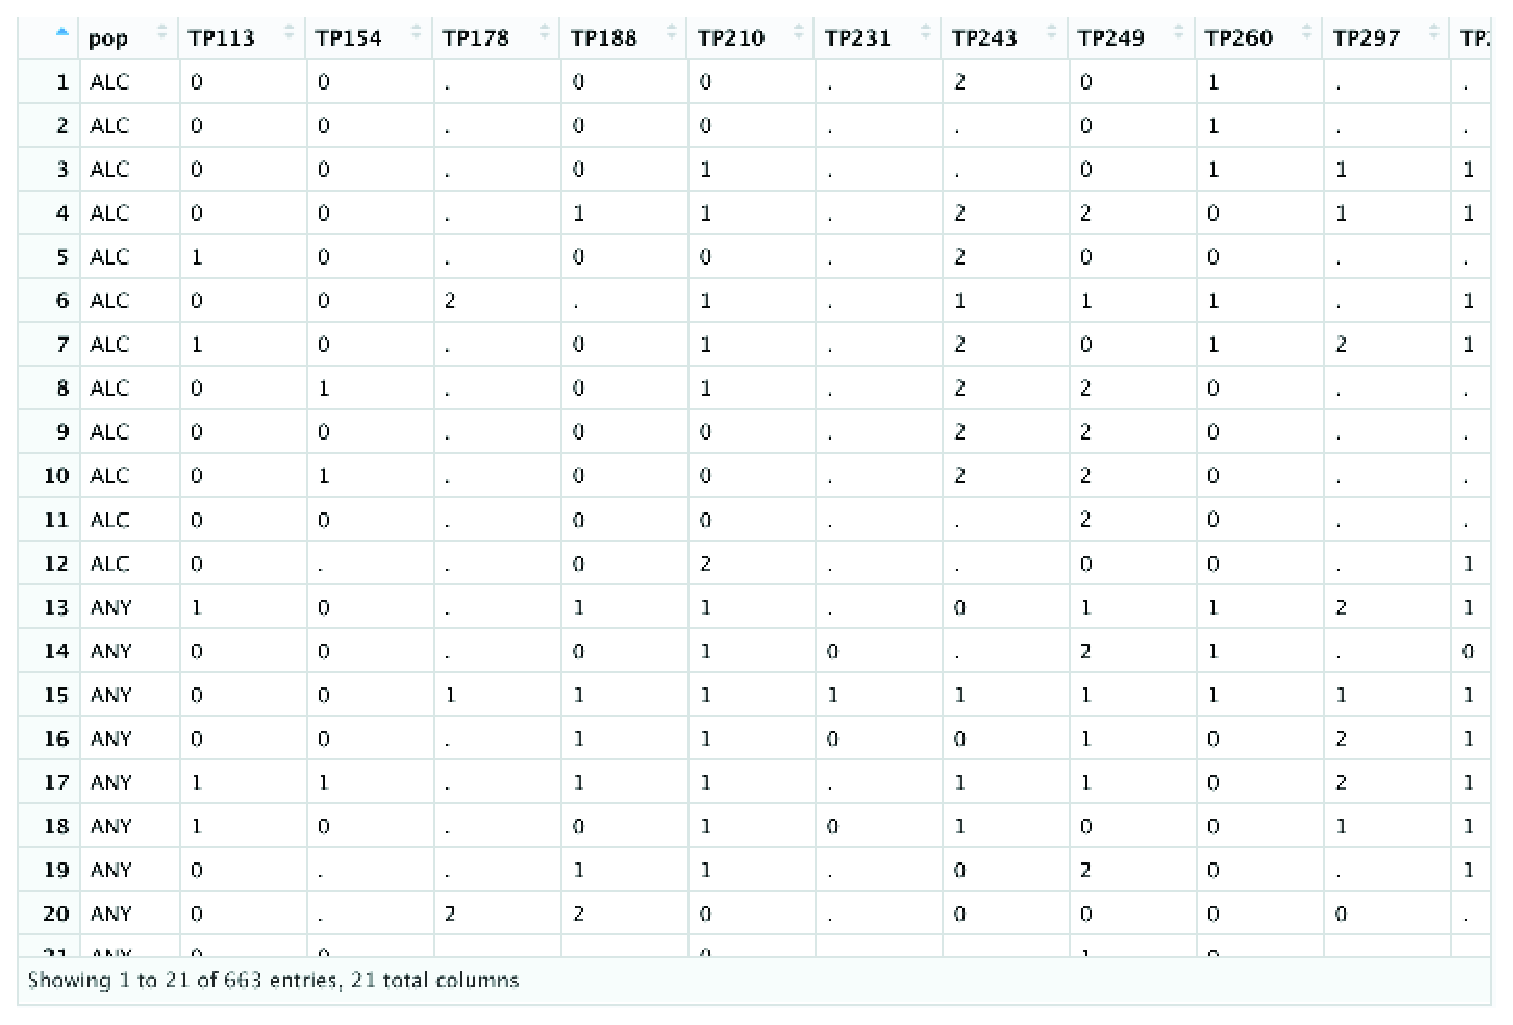
\includegraphics{repens-csv.eps}}
  \end{center}
\caption{Selected rows of a a data set from {\it Protea repens\/} that
  is distributed with {\tt Hickory}~\cite{Prunier-etal-2017}.}\label{fig:repens-csv}
\end{figure}

Now that you understand something about the format of the data that
{\tt Hickory} needs, let's load it into {\tt R} for further analysis.

\begin{verbatim}
genos <- read_marker_data("isotoma.csv")
\end{verbatim}

\subsubsection*{Running the analysis}

Now that the data are loaded, running the analysis is very
straightforward.

\begin{verbatim}
fit <- analyze_codominant(genos)
\end{verbatim}
The results are pretty easy to interpret, too.
{\small
\begin{verbatim}
Inference for Stan model: analyze_codominant.
4 chains, each with iter=2000; warmup=1000; thin=1; 
post-warmup draws per chain=1000, total post-warmup draws=4000.

          mean se_mean    sd     2.5%      25%      50%      75%    97.5% n_eff  Rhat
f        0.344   0.002 0.101    0.147    0.276    0.345    0.414    0.538  3539 1.000
theta    0.075   0.001 0.046    0.017    0.042    0.065    0.096    0.197  1223 1.002
lp__  -121.464   0.150 4.035 -130.283 -124.022 -121.095 -118.549 -114.516   727 1.003

Samples were drawn using NUTS(diag_e) at Sat Jul  3 16:07:48 2021.
For each parameter, n_eff is a crude measure of effective sample size,
and Rhat is the potential scale reduction factor on split chains (at 
convergence, Rhat=1).
\end{verbatim}
}
The column labeled {\tt mean} is the posterior mean for the parameter
listed in the first column.\footnote{Don't worry about {\tt lp\_\_}
for the time being.} The column labeled {\tt se\_mean} is the standard
error of the mean. It's a measure of how accurate the estimate of the
posterior mean is, and we want it to be very small relative to the
estimate of the posterior mean. The column labeled {\tt sd} is the
standard deviation of the posterior mean. It's a measure of our
uncertainty about the mean. We expect about 95\% of the posterior
probability to lie within 2 standard deviations of the mean. If we
compare the 2.5\% and 97.5\% quantiles,\footnote{Corresponding to 95\%
  of the posterior probabiity.} they are very close to what we expect.

In short, there appears to be a reasonable amount of inbreeding within
populations ($f = 0.344$) and a small to moderate amount of among
population differentiation ($\theta = 0.075$). In contrast to the Weir
and Cockerham method, we also have estimates of uncertainty associated
with both $f$ and $\theta$.\footnote{It's not too difficult to get
  estimates of uncertainty using the Weir and Cockerham approach, but
  it takes some additional work.} Since you've probably forgotten what
the other estimates look like, Table~\ref{table:hickory-comparison}
compares all of the approaches we've considered.

\begin{table}
\begin{center}
  \begin{tabular}{c|ll}
\hline\hline
Method & $F_{is}$ & $F_{st}$ \\
\hline
Direct            & 0.137 & 0.214 \\
Nei               & 0.309 & 0.240 \\
Weir \& Cockerham & 0.540 & 0.039 \\
{\tt Hickory}     & 0.344 & 0.075 \\
\hline
\end{tabular}
\end{center}
\caption{Comparison of different approaches for estimating population
  structure from genetic data.}\label{table:hickory-comparison}
\end{table}

The logic behind {\tt Hickory\/} matches the logic behind Weir \&
Cockerham. With moderate to large sample sizes, the point estimates
are reasonably close. They're somewhat different here because there is
only one locus in the sample and because the sample sizes in some of
the populations are very small. Notice, however, that the {\tt
  Hickory} and the Weir \& Cockerham estimates are similar in one very
important respect. The estimate of $F_{ST}$ is much smaller in them
than in Nei's method or the direct method because they take account of
genetic sampling, not just statistical sampling.\index{genetic sampling}\index{statistical sampling}

\subsubsection*{Thinking about priors}

When I introduced the Bayesian model I reminded you that we need to
specify priors to complete it, so how did I get away without
specifying any priors in the analysis we just completed? Because {\tt
  Hickory} picks priors by default when you don't specify them. It
picks priors for $f$ and $\theta$ such that there's a 95\% chance that
they lie between 0.01 and 0.2. That makes sense for many organisms,
since many of them are outbreeding and have low to moderate amounts of
population differentiation. If we have a fair amount of data, that
choice won't make much difference. What about here?

Instead of starting our analysis thinking that we have a reasonably
good idea of what $f$ and $\theta$ ought to be, let's suppose we don't
have much of an idea at all. In particular, let's imagine that all
we're willing to say is that there's a 95\% chance that $f$ and
$\theta$ lie between 0.1 and 0.9. How do we incorporate that into the
analysis?

\begin{verbatim}
fit <- analyze_codominant(genos, prior_f = list(lower = 0.1, upper = 0.9), 
                          prior_theta = list(lower = 0.1, upper = 0.9))
\end{verbatim}
As you can see, the results are quite different from those we got
before.

{\small
\begin{verbatim}
Inference for Stan model: analyze_codominant.
4 chains, each with iter=2000; warmup=1000; thin=1; 
post-warmup draws per chain=1000, total post-warmup draws=4000.

          mean se_mean    sd     2.5%      25%      50%      75%    97.5% n_eff  Rhat
f        0.523   0.001 0.094    0.331    0.460    0.525    0.590    0.693  4027 0.999
theta    0.263   0.005 0.131    0.068    0.163    0.243    0.342    0.571   724 1.005
lp__  -122.391   0.184 4.255 -131.796 -125.070 -121.939 -119.311 -115.408   533 1.007

Samples were drawn using NUTS(diag_e) at Sat Jul  3 16:43:51 2021.
For each parameter, n_eff is a crude measure of effective sample size,
and Rhat is the potential scale reduction factor on split chains (at 
convergence, Rhat=1).
\end{verbatim}
}

The posterior mean of $f$ is now $0.523$ rather than $0.344$, and the
posterior mean of $\theta$ is now $0.263$ rather than $0.075$. If
you're following along, you're probably asking yourself ``Which of
those estimates should I believe?'' My advice is that you shouldn't
believe either of them very much. Remember what a Bayesian model looks
like.

$$
\mbox{P}(\phi|x) = \frac{\mbox{P}(x|\phi)\mbox{P}(\phi)}{\mbox{P}(x)}
$$

\noindent We get the posterior mean from the posterior distribution,
$\mbox{P}(\phi|x)$. If the posterior mean changes substantially based
on different choices for the prior, $\mbox{P}(\phi)$, it means that we
don't have enough data for the likelihood, $\mbox{P}(x|\phi)$ to
dominate the result. In simpler terms, if different choices for the
prior lead to markedly different conclusions, our confidence in those
conclusions depends heavily on our prior beliefs, not just the data
we've collected. Unless we have a lot of confidence in our prior
beliefs, we shouldn't have much confidence in the conclusions.

One of the nice things about a Bayesian approach is that it gives us a
straightforward way to assess how much to rely on inferences from the
data we've collected. If different priors have a large influence on
the posterior, as they do here, it tells us that the data we've
collected don't have much information about the parameters we're
interested in. If different priors don't have a large influence, then
the data {\it do\/} have a fair amount of information about the
parameters.\footnote{If it seems as if I'm repeating myself, I
  probably am, but I think this is a really immportant point that
  bears repeating.} 

There's a general lesson here: Think carefully about the prior
distribution on the parameters in {\it any\/} Bayesian model you use,
{\it and\/} consider exploring at least a couple of different choices
of priors to see if they have a large influence on your
conclusions. In addition, {\it pay attention to the credible
  intervals}. In both sets of analyses you've just seen, the credible
intervals are very wide. That in itself says that the data aren't
giving you a very clear idea of what the parameter is.

\subsection*{Assessing evidence for inbreeding and population
  differentiation}

You've already seen that {\tt Hickory} gives you estimates of the
credible intervals for $f$ and $\theta$, but if you're interested in
seeing whether there is evidence for inbreeding within populations or
for genetic differentiation among populations, you can't just look to
see whether the credible intervals overlap $0$. Why? because $f$ and
$\theta$ are defined to lie between 0 and 1 in {\tt Hickory} so they
can't overlap 0.\footnote{We noted a couple of lectures ago that $f$
  can be negative when it's understood as a measure of departure from
  Hardy-Weinberg, but for computational reasons, {\tt Hickory}
  restricts it to $[0,1]$. If you're interested in the gory details of
  why, feel free to ask me.} In some data sets the posterior mean for
either or both may be substantially larger than 0, and the lower bound
of the credible interval may also be substantially larger than 0. In
such cases, you'd be pretty safe saying that you have evidence for
inbreeding or geographical differentiation, but what if you have a
situation like what you get from using the {\it Protea repens\/} data
set that is distributed with {\tt Hickory}.

{\small
\begin{verbatim}
genos <- read_marker_data(system.file("extdata", "protea_repens.csv", package = "Hickory"))
fit <- analyze_codominant(genos)

Inference for Stan model: analyze_codominant.
4 chains, each with iter=2000; warmup=1000; thin=1; 
post-warmup draws per chain=1000, total post-warmup draws=4000.

           mean se_mean     sd      2.5%       25%       50%       75%     97.5% n_eff  Rhat
f         0.005   0.000  0.002     0.002     0.003     0.005     0.006     0.010  5169 0.999
theta     0.081   0.000  0.008     0.066     0.075     0.081     0.086     0.097  1599 1.001
lp__  -6242.725   0.538 17.416 -6276.812 -6254.305 -6242.781 -6230.561 -6209.327  1048 1.005

Samples were drawn using NUTS(diag_e) at Sun Jul  4 12:52:05 2021.
For each parameter, n_eff is a crude measure of effective sample size,
and Rhat is the potential scale reduction factor on split chains (at 
convergence, Rhat=1).
\end{verbatim}
}

The posterior means and credible intervals in these data are
relatively insensitive to our choice of priors.\footnote{Don't take my
  word for it. Run the analysis yourself with the second set of priors
  we used above or with another set of priors that strikes your fancy
  and compare the results.} The posterior mean for $\theta$ is only
0.081, but the lower bound of the 95\% credible interval is 0.066 and
the credible interval is quite small, which gives us reasonably strong
evidence that $\theta > 0$, i.e., that there is genetic
differentiation among populations. But what about inbreeding within
populations? The posterior mean of $f$ is only 0.005, and the lower
bound of the 95\% credible interval is barely greater than 0, i.e.,
0.002. That doesn't seem like very good evidence either way, but can
we say something more?\footnote{Would I be asking this question if the
  answer were ``No''?}

We could simply do Hardy-Weinberg tests at every locus in every
population, but that could get pretty tedious. If we did that, we'd
also run into problems with multiple tests, which are inconvenient to
deal with. We'll take a different approach. Namely, we'll compare the
model we just fit with one that {\it assumes\/} there is no inbreeding
within populations, i.e., $f = 0$. The criterion we'll use to compare
the models is something known as the expected log predictive
density~\cite{Vehtari-etal-2017}. That's a mouthful, and the
mathematics is reasonably complicated, but it's easy enough to
interpret the results without understanding all of those details.

First, we run the model in which we assume $f = 0$ and store the
result in a different object.
\begin{verbatim}
fit_f0 <- analyze_codominant(genos, f_zero = TRUE)

Inference for Stan model: analyze_codominant.
4 chains, each with iter=2000; warmup=1000; thin=1; 
post-warmup draws per chain=1000, total post-warmup draws=4000.

           mean se_mean     sd      2.5%       25%       50%       75%     97.5% n_eff  Rhat
f         0.000     NaN  0.000     0.000     0.000     0.000     0.000     0.000   NaN   NaN
theta     0.081   0.000  0.008     0.067     0.076     0.080     0.086     0.097  1934 1.000
lp__  -6234.006   0.518 16.882 -6267.340 -6245.573 -6233.842 -6222.445 -6202.017  1060 1.001

Samples were drawn using NUTS(diag_e) at Sun Jul  4 13:21:39 2021.
For each parameter, n_eff is a crude measure of effective sample size,
and Rhat is the potential scale reduction factor on split chains (at 
convergence, Rhat=1).
\end{verbatim}
Notice that the estimate for $f$ is 0, as expected. Now we can
compare the two models using {\tt loo()}.\footnote{I call the first
  object {\tt loo\_free} because in that model $f$ was free to vary.}
\begin{verbatim}
loo_free <- loo(fit)
loo_f0 <- loo(f0)
compare(loo_free, loo_f0)
\end{verbatim}
You'll see some warning messages when you run {\tt loo()} with these
data. In an ideal world, we'd do things a bit differently and get rid
of them, but in this case, we don't need to worry about them. Let's
focus on the table that was printed.
\begin{verbatim}
       elpd_diff se_diff
model2  0.0       0.0   
model1 -1.8       3.4   
\end{verbatim}
The column labeled {\tt elpd\_diff} is the difference in expected log
predictive density between the model with the highest elpd and the
model on the line in which the entry appears. The column labeled {\tt
  se\_diff} is the standard error of that difference. {\tt model 2}
refers to the second model named in the call to {\tt compare()}, i.e.,
the $f=0$ model ({\tt loo\_f0}), and {\tt model 1} refers to the first
model named in the call to {\tt compare()}, i.e., the $f$ ``free''
model. What all of this means is that

\begin{itemize}

  \item Model 2, the $f=0$ model, is more strongly supported than
    Model 1, the model in which we estimated $f$, {\it but}

  \item The difference between the two models, -1.8, is substantially
    less than twice the standard error of the difference (3.4),
    meaning that we don't have good evidence that one model is better
    than the other.
    
\end{itemize}

You may find it dissatisfying that we can't distinguish between these
two models and that we're left saying that we don't know whether we
have evidence for inbreeding within populations or not, but remember,
our estimate of $f$ is only
0.005. Table~\ref{table:f-model-comparison} shows what that means for
expected genotype frequencies if $p = 0.5$. As you can see, the
difference in genotype frequencies is extremely small. It's hard to
believe that there would be any biologically meaningful difference
between any of the scenarios that seem compatible with the data.

\begin{table}
  \begin{center}
    \begin{tabular}{l|lll}
      \hline\hline
      Model       & $A_1A_1$ & $A_1A_2$ & $A_2A_2$ \\
      \hline
      $f = 0$     & 0.25     & 0.50    & 0.25 \\
      $f = 0.005$ & 0.25125  & 0.4975  & 0.25125 \\
      $f = 0.010$ & 0.2525   & 0.495   & 0.2525 \\
      \hline
    \end{tabular}
  \end{center}
  \caption{Comparison of genotype frequencies assuming $p = 0.5$ with
    $f = 0$ and $f$ as estimated (mean and upper bound of the 95\%
    credible interval) from the {\it Protea repens\/} data distributed
    with {\tt Hickory}.}\label{table:f-model-comparison}
\end{table}

\subsection*{Extending the model}

It is relatively straightforward to extend the basic model above to
account for the possibility that the amount of differentiation at some
loci is much greater (or much smaller) than it is as most
loci. Similarly, it is relatively straightfoward to extend the model
to allow some populations to be much more similar to (or much more
different from) the average population allele frequencies than
others. All we need to do is to allow $\theta$ to reflect locus- and
population-specific effects.

\begin{eqnarray*}
  \theta_i &=& \mbox{locus-specific $\theta$} \\
  \theta_k &=& \mbox{population-specific $\theta$} \\
  \theta_{ik} &=& \mbox{population- and locus-specific $\theta$} \\
  &=& (\theta_i + \theta_k)/2 \quad .
\end{eqnarray*}
You can read more about estimating locus- and population-specific
effects in the documentation for {\tt Hickory} if you're interested.

